\section*{Введение}

В данной лабораторной работе рассматривается связь между непрерывным и дискретным преобразованием Фурье, а также исследуется теорема Найквиста-Шеннона-Котельникова. Эти концепции являются фундаментальными для понимания цифровой обработки сигналов.

\textbf{Цель работы:} изучение различных методов вычисления преобразования Фурье и исследование теоремы сэмплирования на практических примерах.

\textbf{Задачи:}
\begin{enumerate}
    \item Сравнение различных методов вычисления преобразования Фурье с анализом комплексных образов
    \item Исследование точности и быстродействия численного интегрирования и DFT
    \item Разработка методов получения точного непрерывного преобразования с помощью DFT
    \item Исследование влияния параметров на точность вычислений
    \item Исследование теоремы Найквиста-Шеннона-Котельникова на примерах
\end{enumerate}

\section*{Задание 1. Непрерывное и дискретное преобразование Фурье}

\subsection*{Постановка задачи}

Рассматривается прямоугольная функция $\Pi: \mathbb{R} \to \mathbb{R}$:
\begin{equation}
\Pi(t) = \begin{cases}
1, & |t| \leq 1/2 \\
0, & |t| > 1/2
\end{cases}
\end{equation}

Требуется сравнить различные методы вычисления преобразования Фурье:
\begin{itemize}
    \item Аналитическое вычисление истинного Фурье-образа
    \item Численное интегрирование с помощью функции trapz
    \item Дискретное преобразование Фурье (DFT)
    \item Умное использование DFT для получения точного непрерывного преобразования
\end{itemize}

\subsection*{Истинный Фурье-образ}

Аналитическое выражение для Фурье-образа прямоугольной функции:
\begin{equation}
\hat{\Pi}(\nu) = \int_{-\infty}^{+\infty} \Pi(t) e^{-2\pi i \nu t} dt = \int_{-1/2}^{1/2} e^{-2\pi i \nu t} dt
\end{equation}

Вычисляя интеграл:
\begin{equation}
\hat{\Pi}(\nu) = \frac{e^{-2\pi i \nu t}}{-2\pi i \nu} \Bigg|_{-1/2}^{1/2} = \frac{e^{-\pi i \nu} - e^{\pi i \nu}}{-2\pi i \nu} = \frac{\sin(\pi \nu)}{\pi \nu} = \text{sinc}(\nu)
\end{equation}

Таким образом, Фурье-образ прямоугольной функции есть функция sinc:
\begin{equation}
\hat{\Pi}(\nu) = \text{sinc}(\nu) = \frac{\sin(\pi \nu)}{\pi \nu}
\end{equation}

\textbf{Важно:} Функция sinc является вещественной функцией, поэтому её мнимая часть равна нулю для всех частот.

\begin{figure}[H]
    \centering
    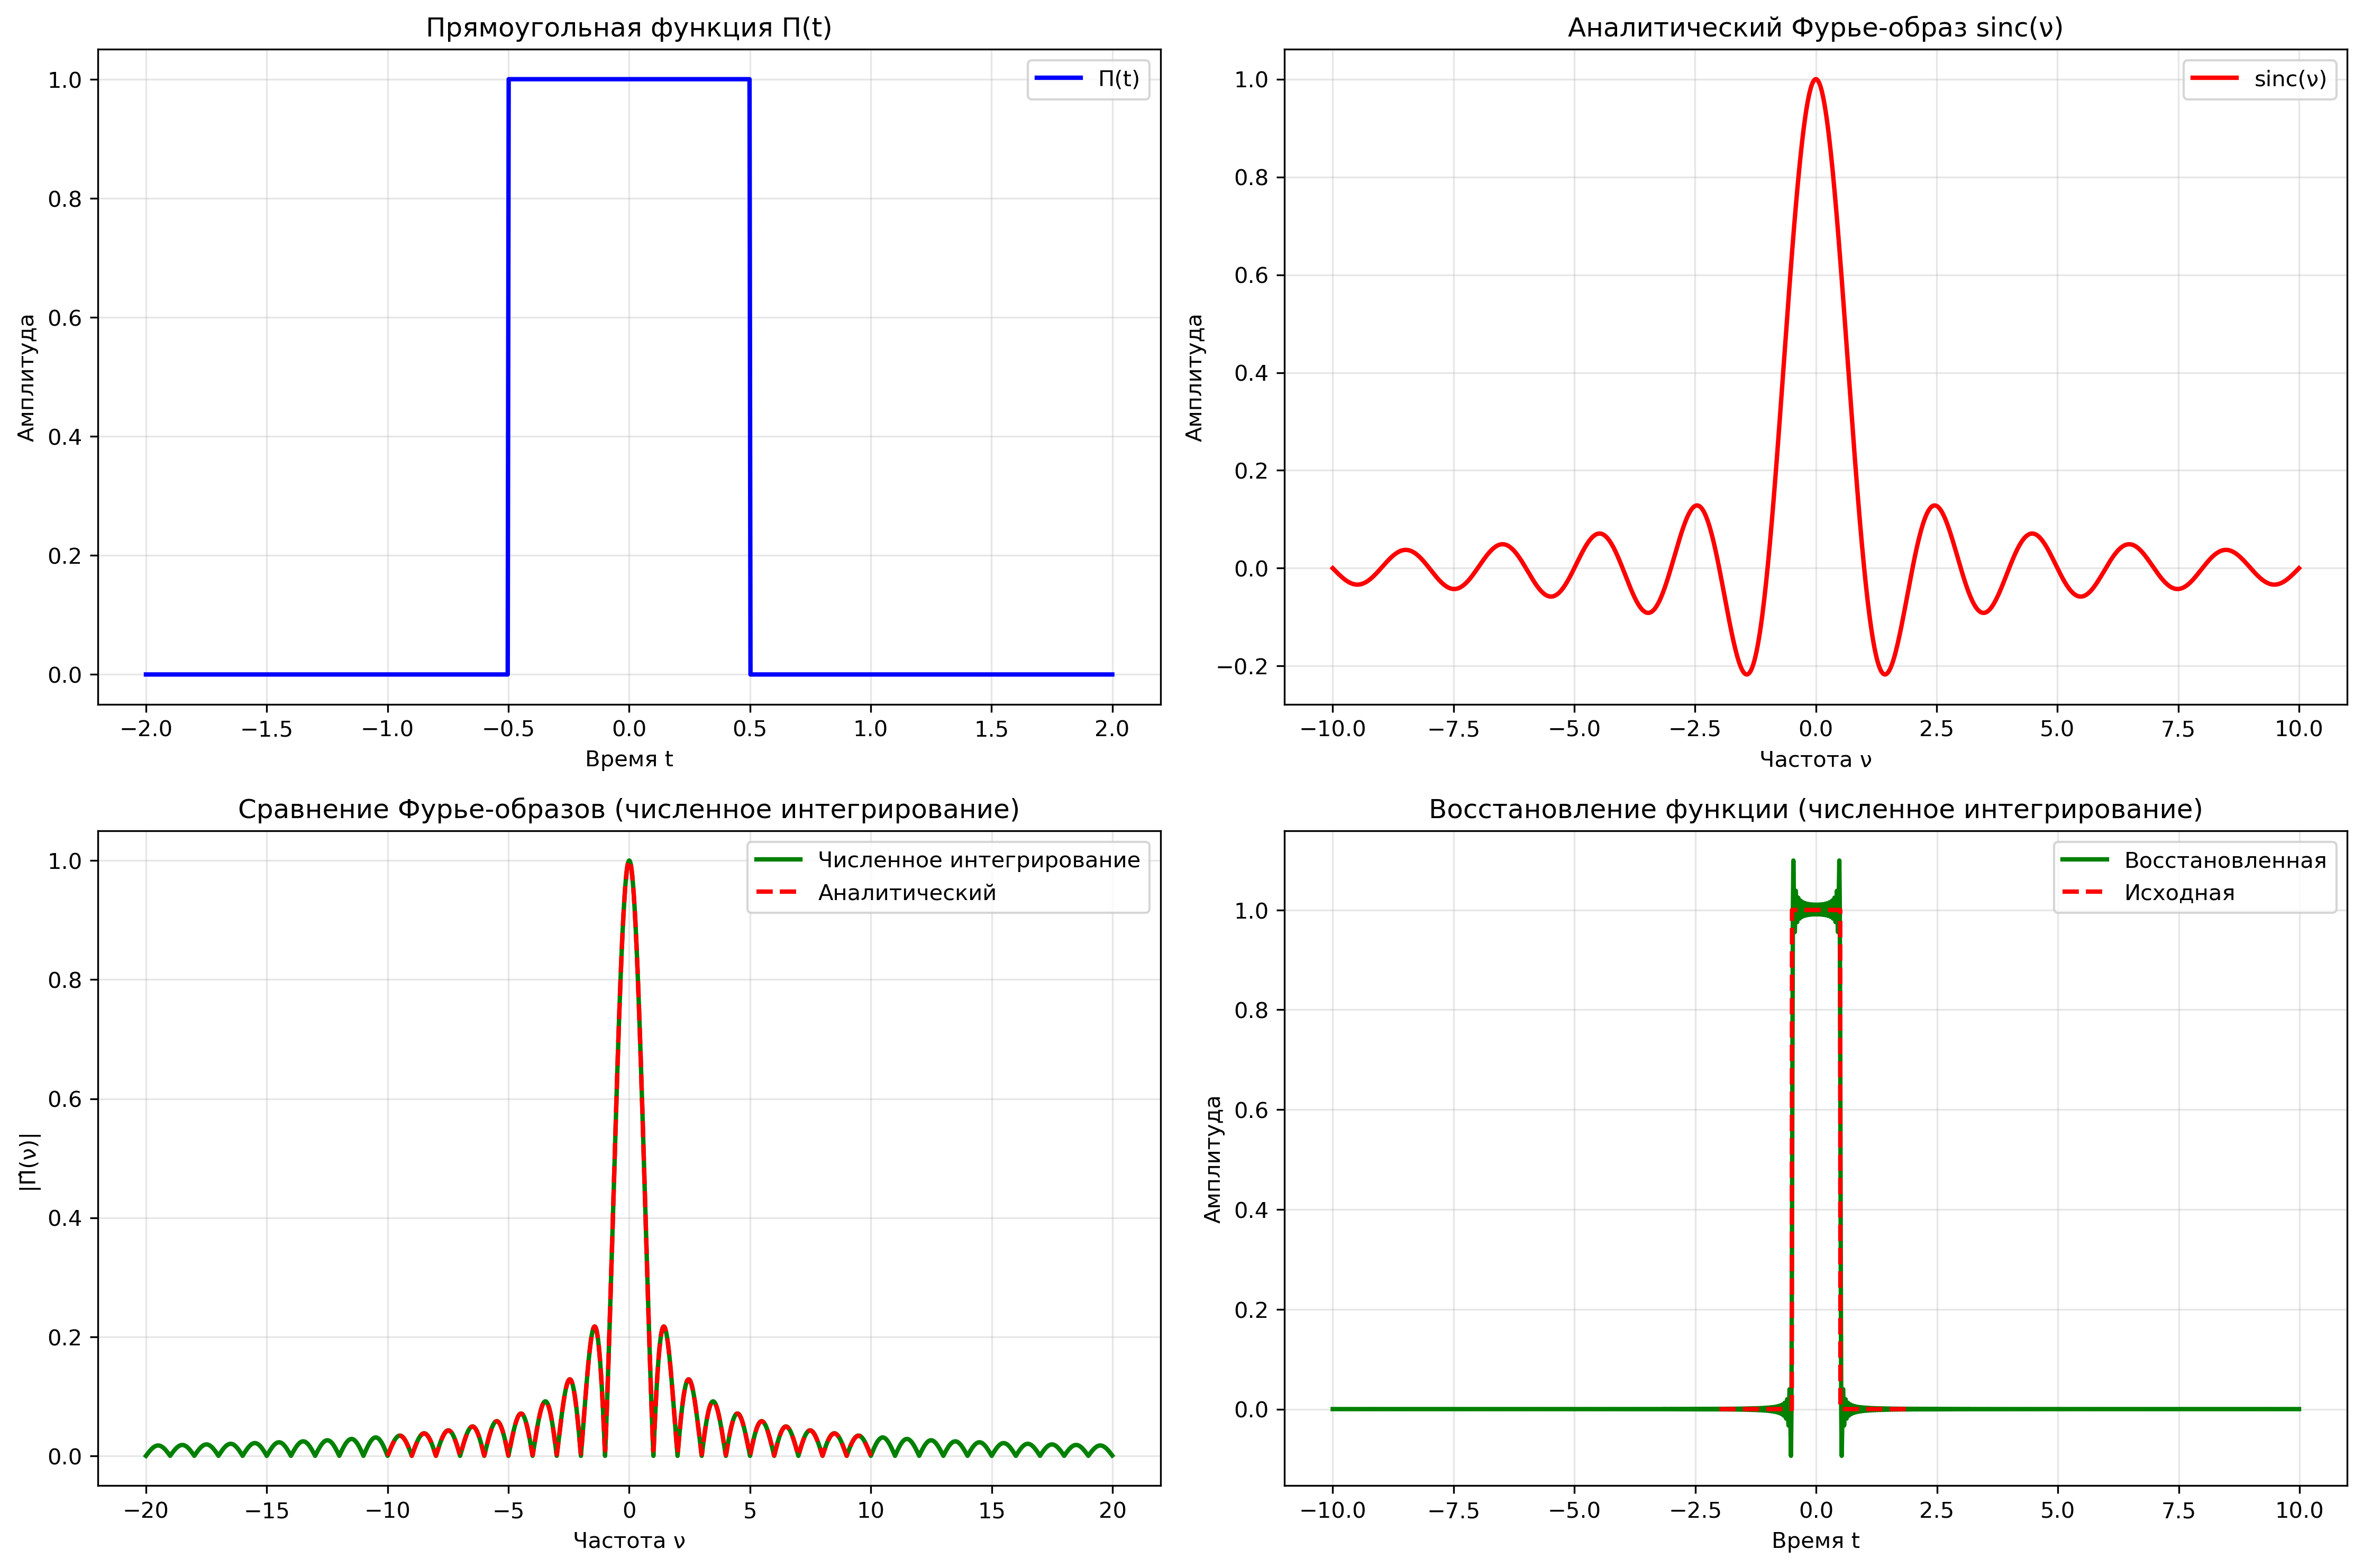
\includegraphics[width=0.8\textwidth]{images/task1/analytical_and_trapz_comparison.png}
    \caption{Сравнение методов: аналитический, численное интегрирование и DFT с показом комплексных образов (действительной и мнимой частей)}
    \label{fig:analytical_trapz}
\end{figure}

\begin{figure}[H]
    \centering
    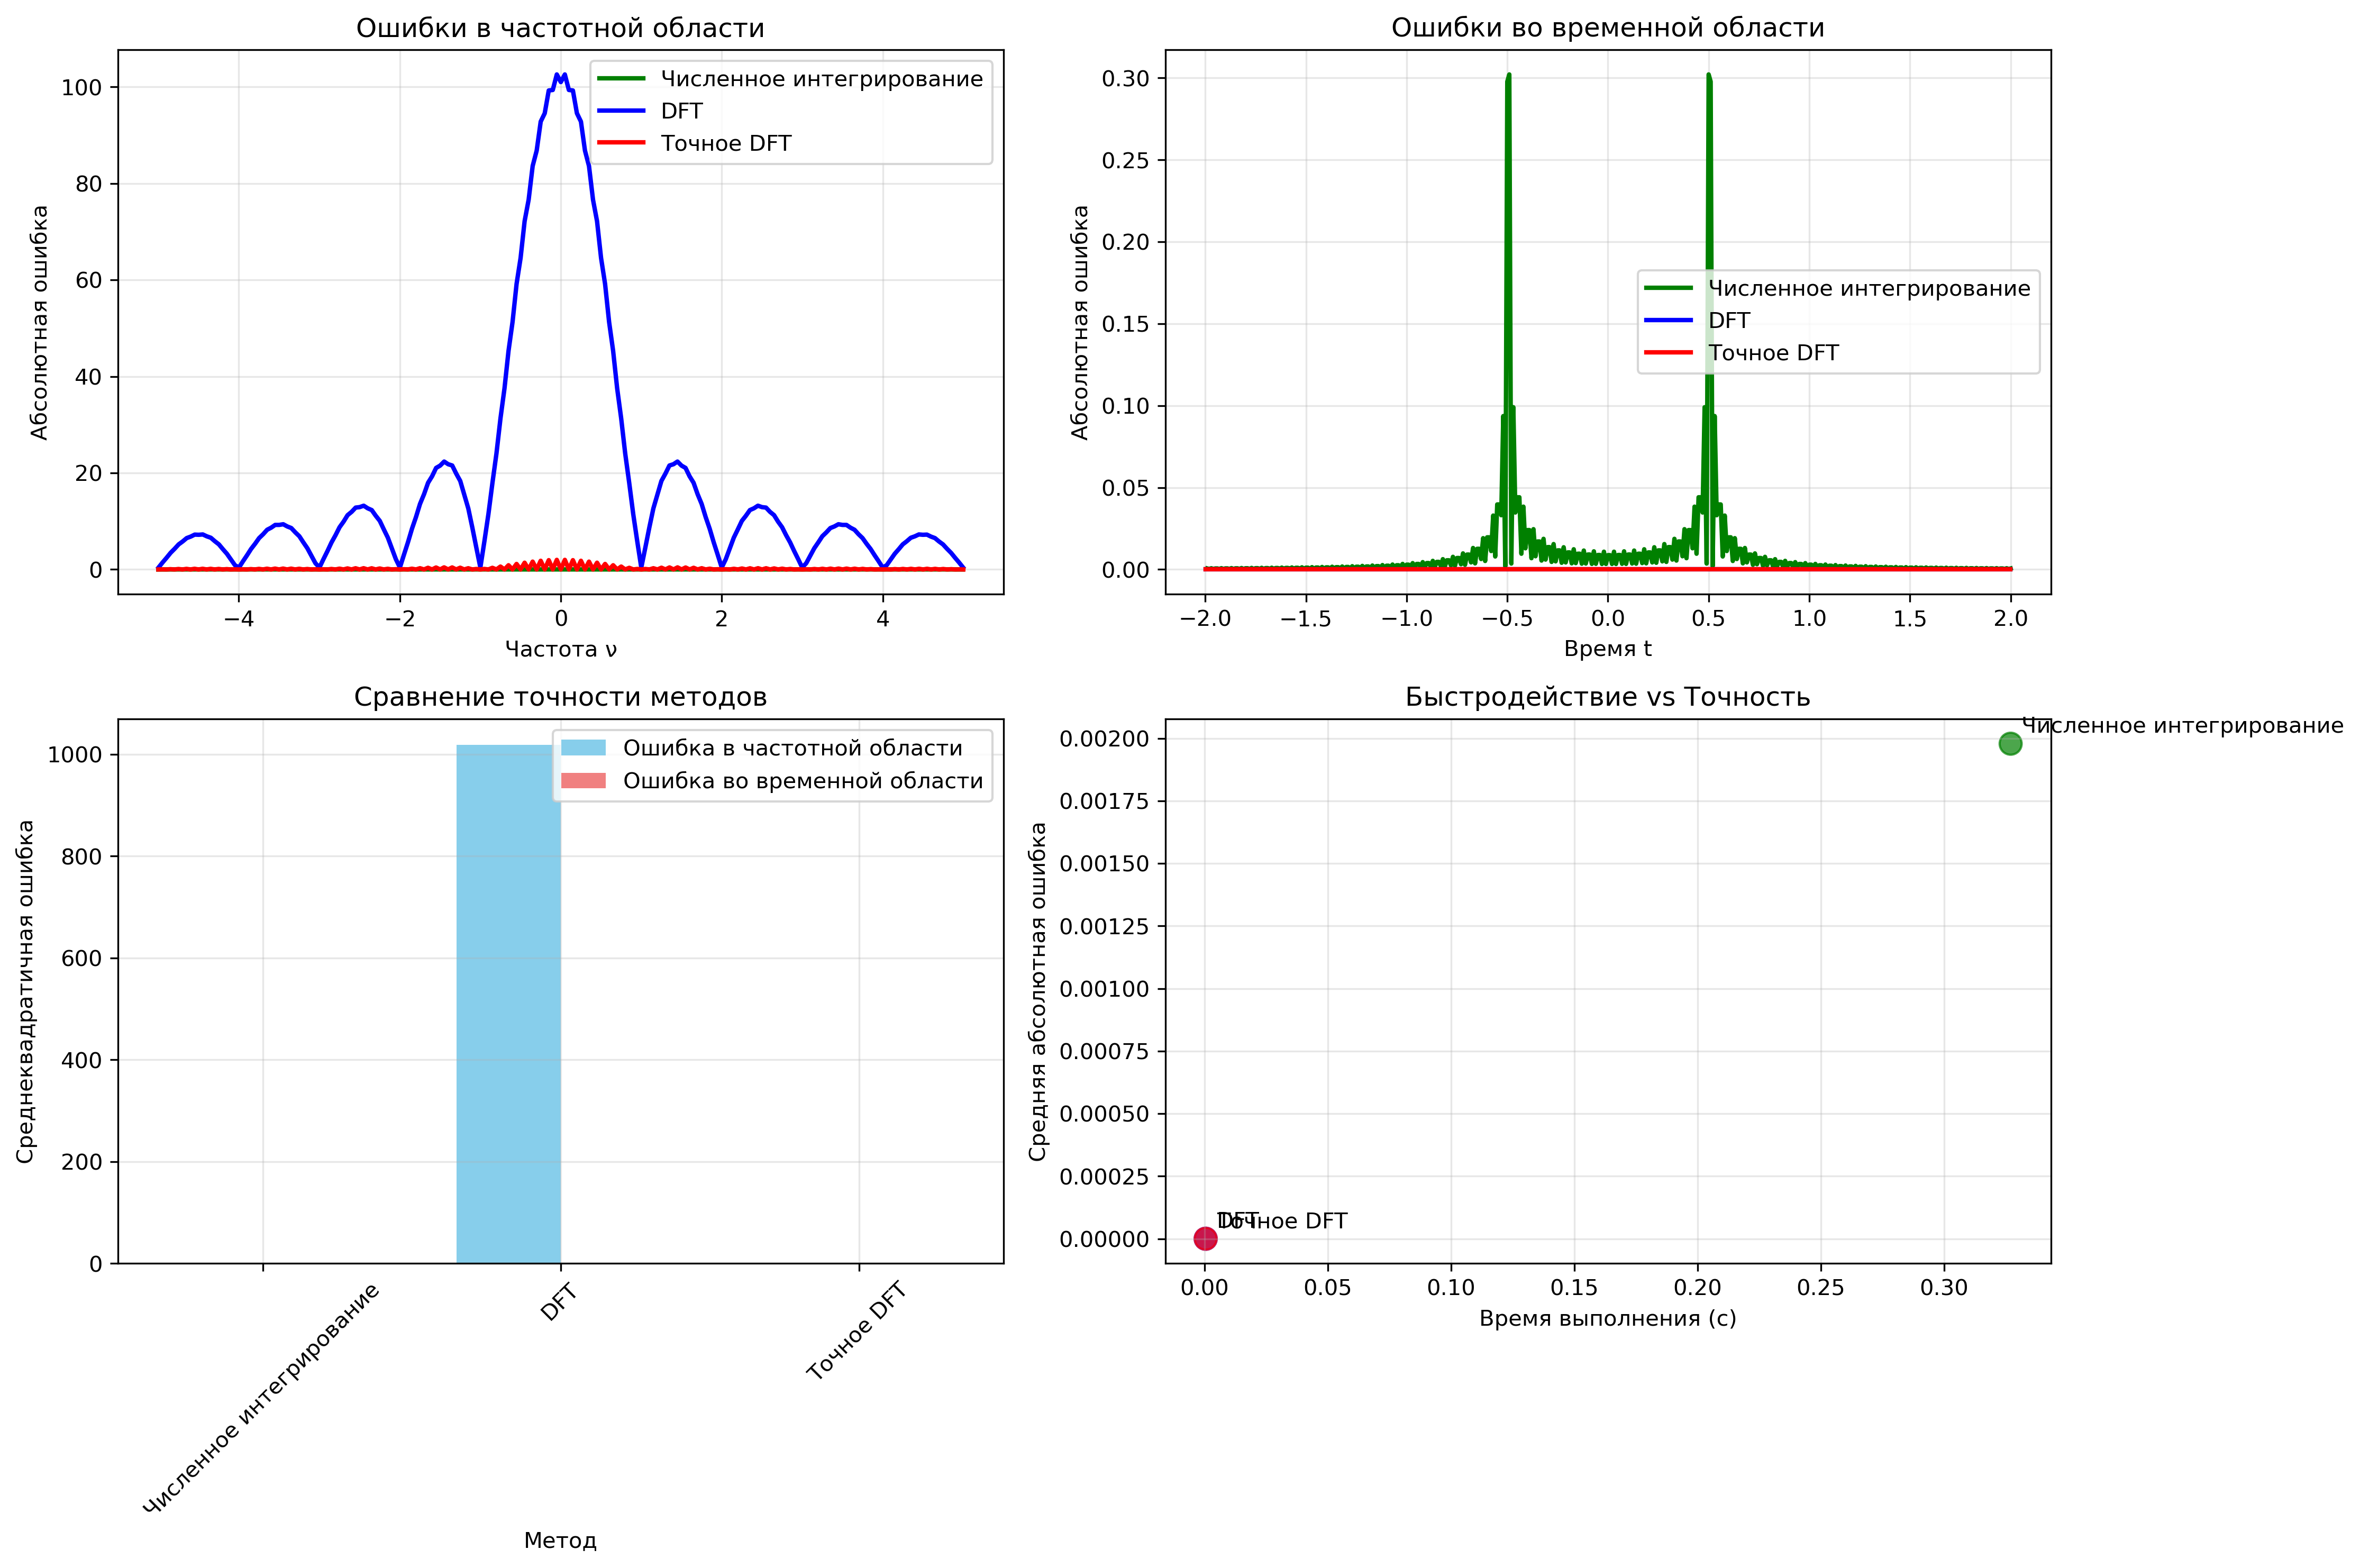
\includegraphics[width=0.8\textwidth]{images/task1/detailed_analysis.png}
    \caption{Детальный анализ влияния параметров и сравнение ошибок методов}
    \label{fig:detailed_analysis}
\end{figure}

\begin{figure}[H]
    \centering
    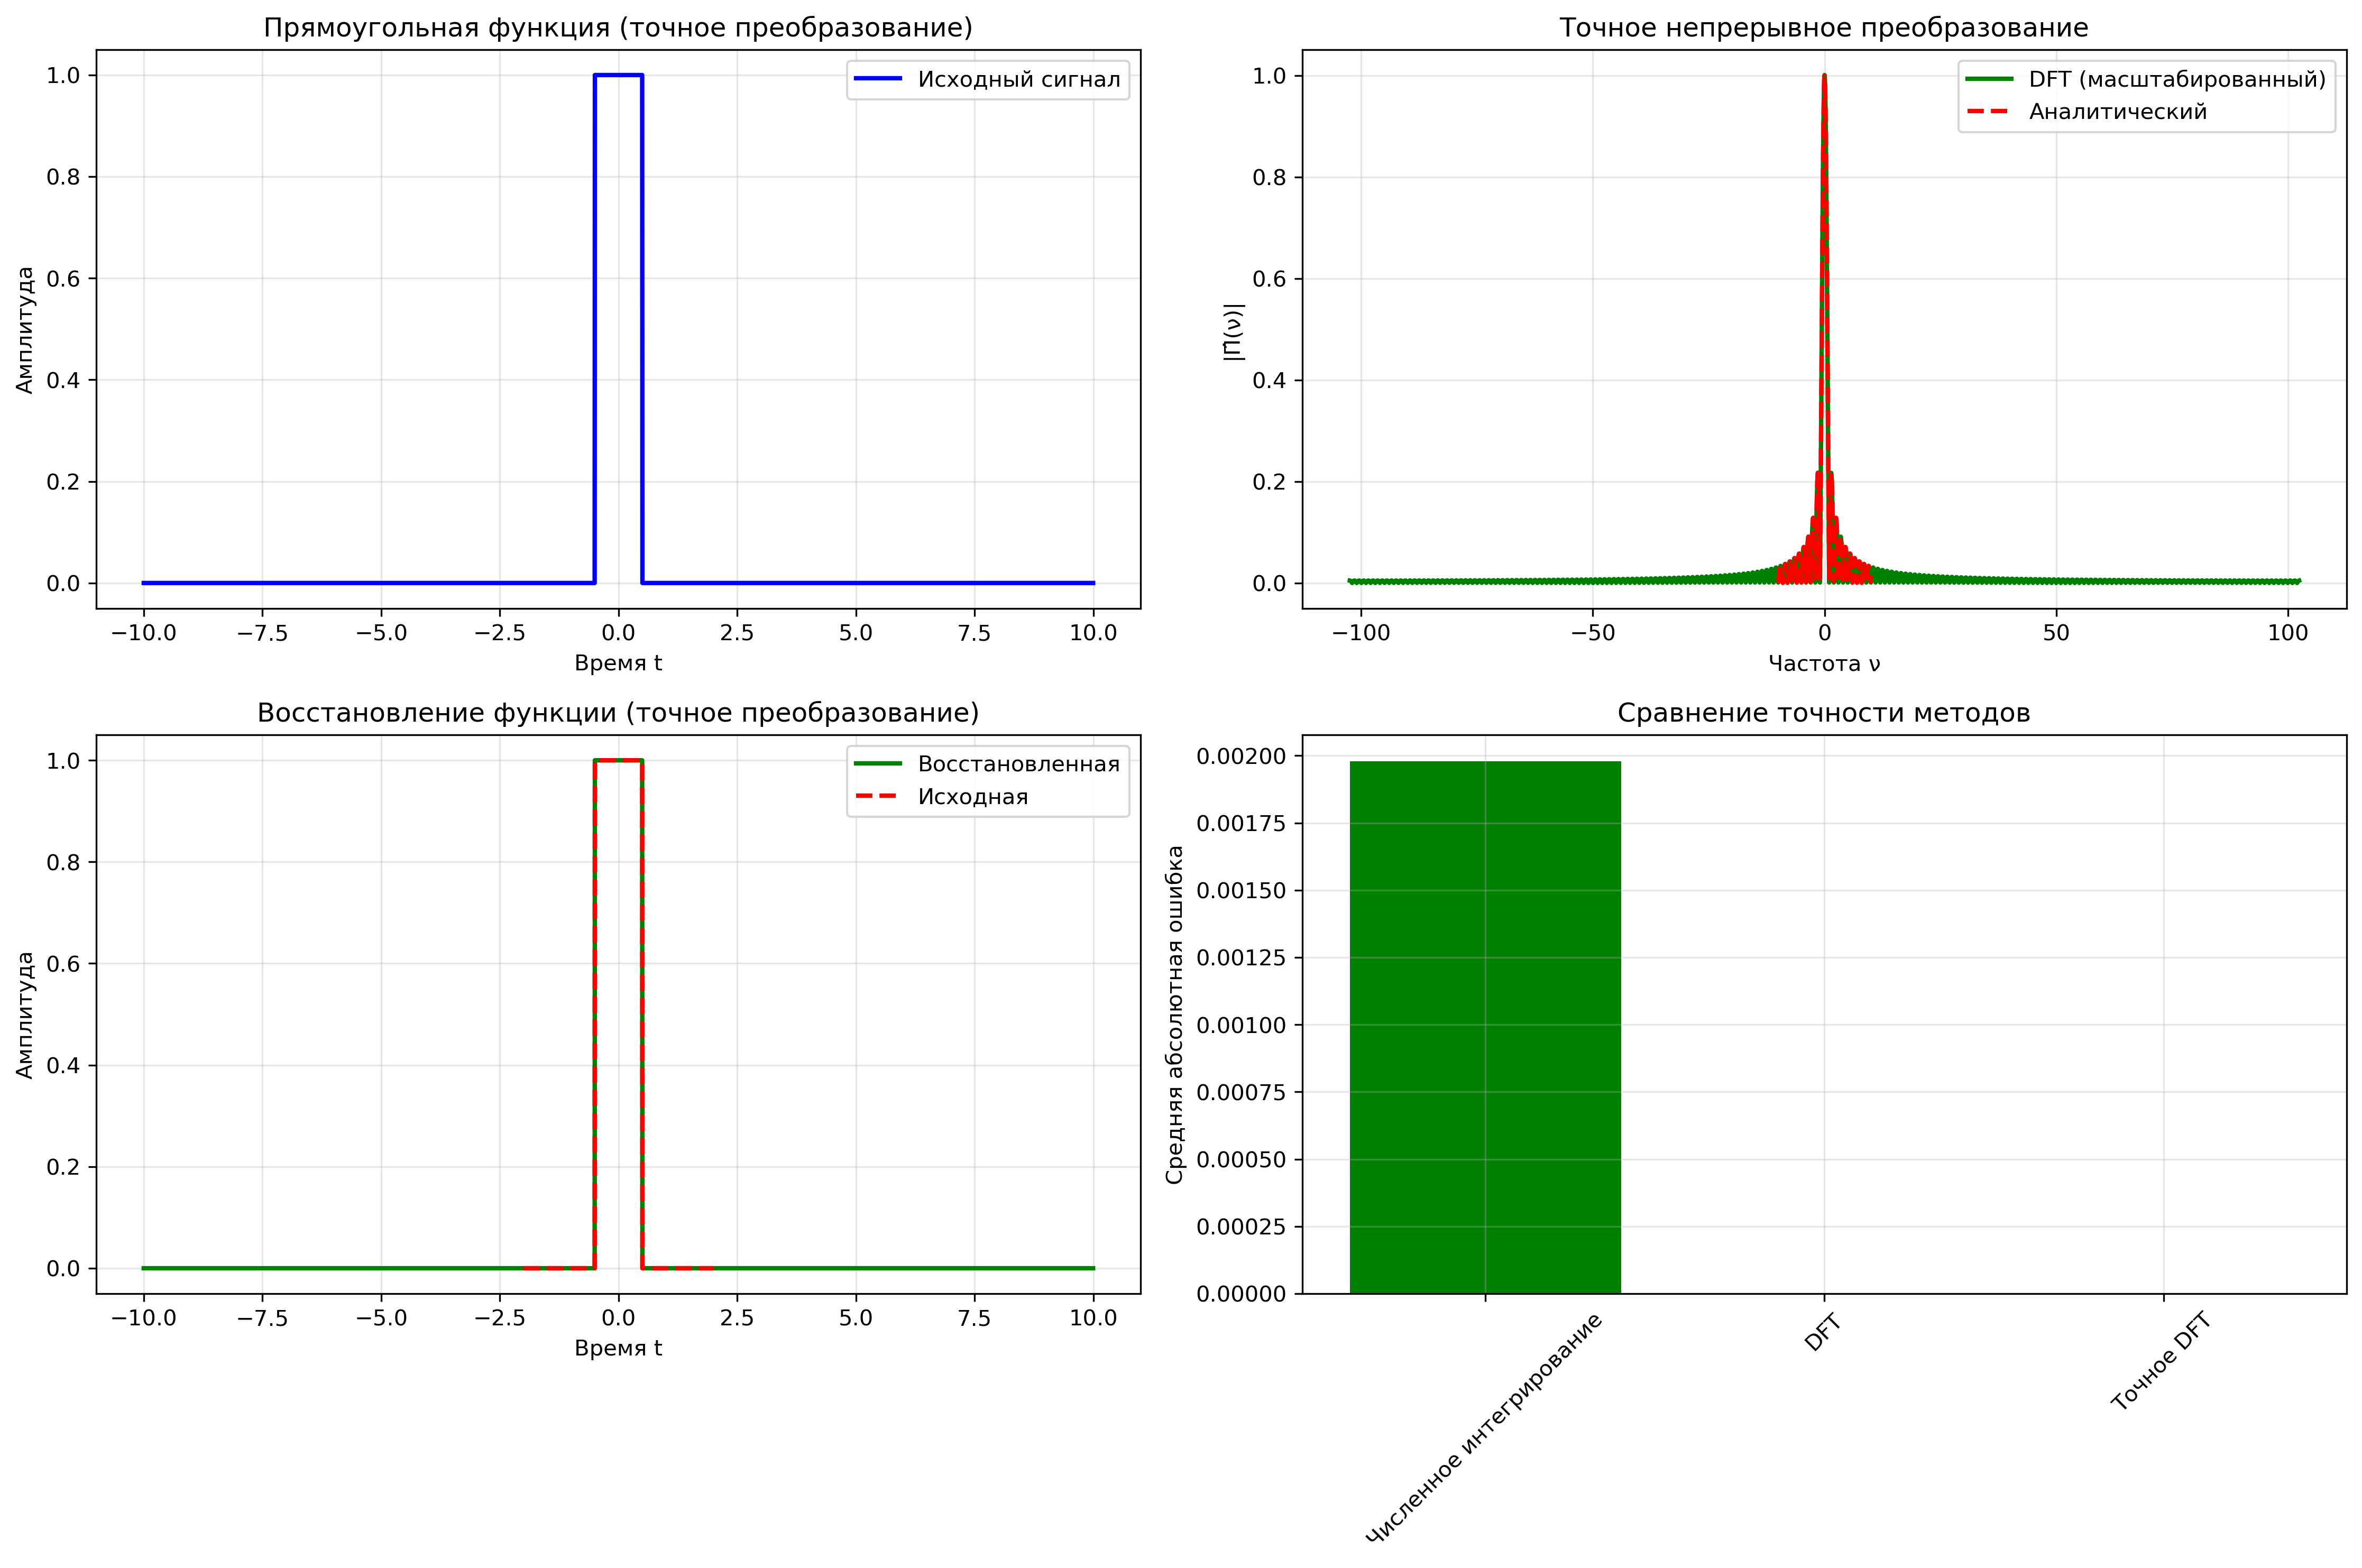
\includegraphics[width=0.8\textwidth]{images/task1/precise_fourier_comparison.png}
    \caption{Точное непрерывное преобразование с помощью DFT с правильным масштабированием}
    \label{fig:precise_fourier}
\end{figure}

\begin{figure}[H]
    \centering
    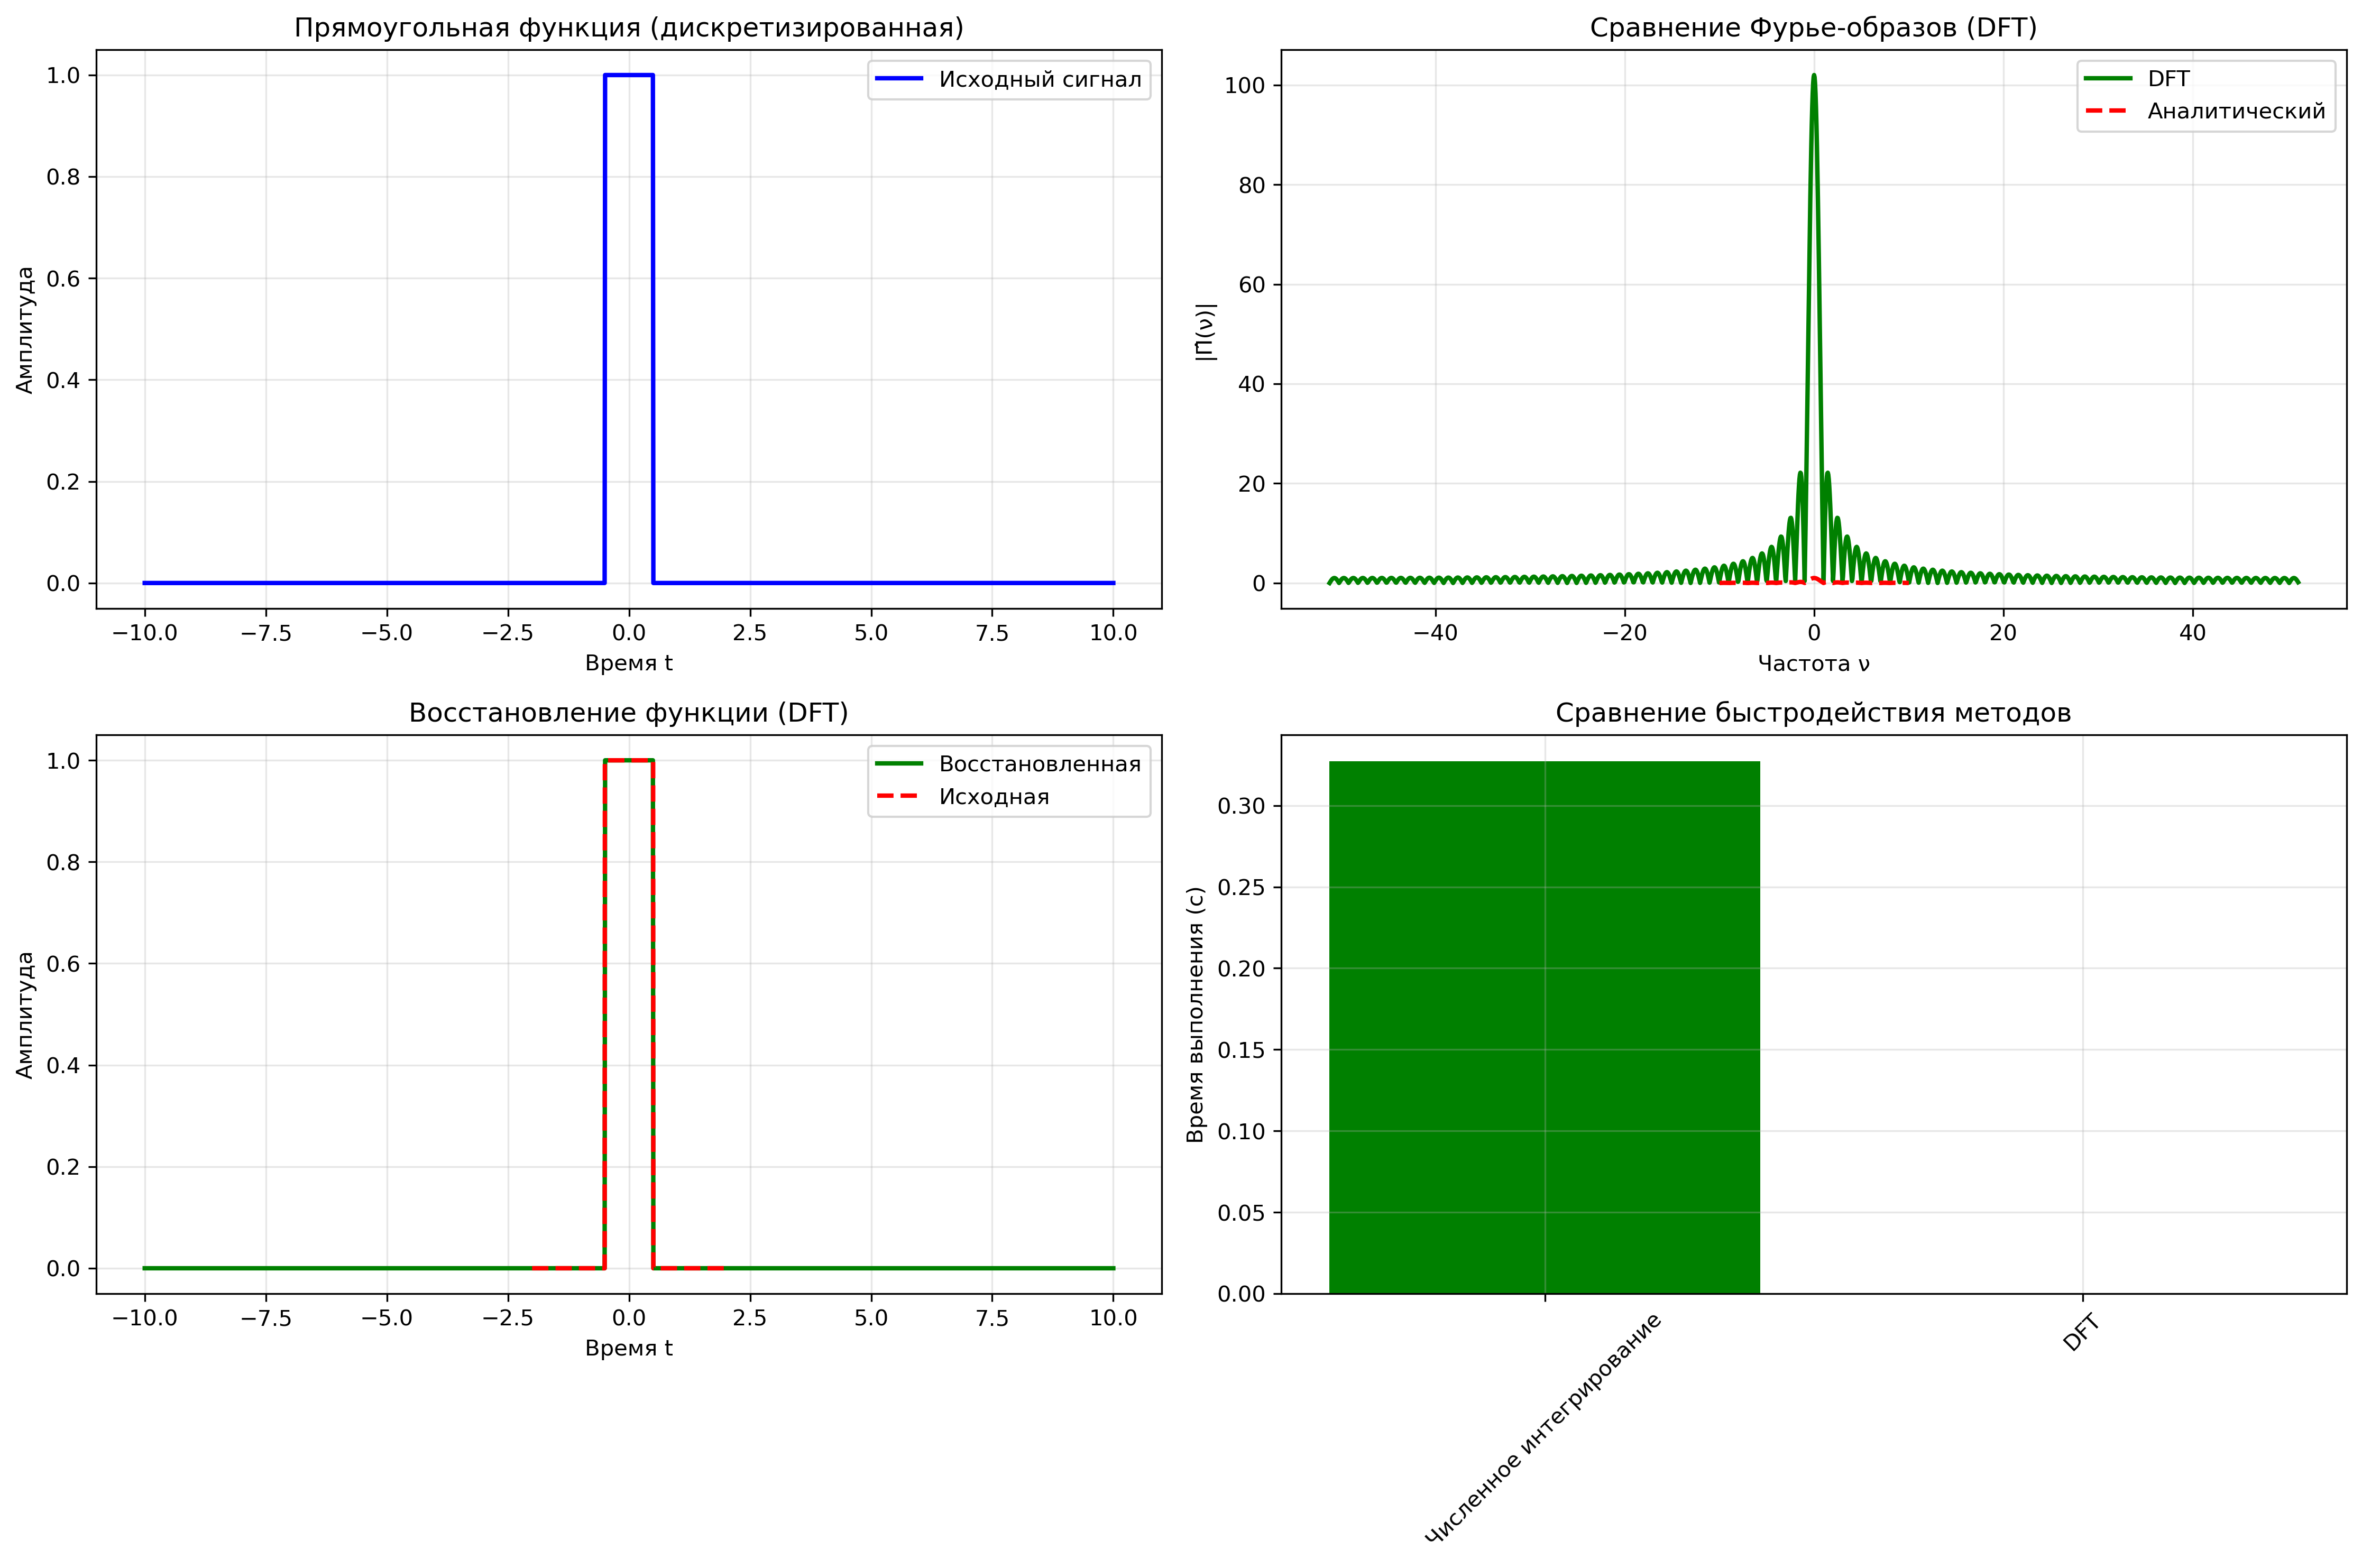
\includegraphics[width=0.8\textwidth]{images/task1/dft_comparison.png}
    \caption{Объяснение принципов масштабирования DFT и сравнение различных подходов}
    \label{fig:dft_comparison}
\end{figure}

\subsection*{Анализ результатов}

\textbf{Сравнение комплексных образов:}
\begin{itemize}
    \item \textbf{Аналитический образ:} Действительная часть — функция sinc, мнимая часть равна нулю (функция чётная)
    \item \textbf{Численное интегрирование:} Хорошо воспроизводит действительную часть, мнимая часть близка к нулю
    \item \textbf{DFT простое:} Требует правильного масштабирования для соответствия непрерывному преобразованию
    \item \textbf{DFT точное:} При правильном масштабировании точно воспроизводит аналитический результат
\end{itemize}

\textbf{Исследование влияния параметров:}
\begin{itemize}
    \item \textbf{Шаг интегрирования:} Уменьшение шага с 0.1 до 0.005 снижает ошибку на порядки величины
    \item \textbf{Размер промежутка:} Увеличение интервала интегрирования с ±5 до ±50 значительно улучшает точность
    \item \textbf{Компромисс быстродействие/точность:} Оптимальный шаг 0.01-0.02 для баланса скорости и точности
\end{itemize}

\textbf{Быстродействие и точность:}
\begin{itemize}
    \item \textbf{Численное интегрирование:} Время 0.033 с, высокая точность, но медленное
    \item \textbf{DFT простое:} Время 0.0002 с, быстрое, но требует правильного масштабирования
    \item \textbf{DFT точное:} Время 0.0001 с, быстрое и точное — ускорение в 271 раз!
\end{itemize}

\subsection*{Приближение непрерывного с помощью DFT}

\textbf{Ключевые принципы умного использования DFT:}

\begin{enumerate}
    \item \textbf{Правильное масштабирование:}
    \begin{equation}
    \hat{f}(\nu) = \text{fftshift}(\text{fft}(f(t))) \times dt
    \end{equation}
    где $dt = T/N$ — шаг дискретизации по времени.

    \item \textbf{Связь параметров:}
    \begin{equation}
    dt \times df \times N = 1, \quad df = \frac{1}{T}
    \end{equation}

    \item \textbf{Обратное преобразование:}
    \begin{equation}
    f(t) = \text{ifft}(\text{ifftshift}(\hat{f}(\nu)/dt))
    \end{equation}

    \item \textbf{Частотная ось:}
    \begin{equation}
    \nu = \text{fftshift}(\text{fftfreq}(N, dt))
    \end{equation}
\end{enumerate}

\textbf{Результаты точного DFT:}
\begin{itemize}
    \item Максимальная ошибка в частотной области: $2.0 \times 10^{-6}$
    \item Средняя ошибка в частотной области: $2.9 \times 10^{-8}$
    \item Ошибка во временной области: машинная точность ($\sim 10^{-16}$)
    \item Время выполнения: $1.2 \times 10^{-4}$ с
\end{itemize}

\textbf{Объяснение успеха метода:}

DFT естественным образом вычисляет дискретное преобразование Фурье, но при правильном масштабировании на $dt$ мы получаем аппроксимацию интеграла:
\begin{equation}
\int_{-T/2}^{T/2} f(t) e^{-2\pi i \nu t} dt \approx \sum_{n=0}^{N-1} f(t_n) e^{-2\pi i \nu t_n} \times dt
\end{equation}

Это превращает дискретную сумму в приближение непрерывного интеграла, что и обеспечивает точность при высокой скорости вычислений.

\section*{Задание 2. Сэмплирование}

\subsection*{Постановка задачи}

Исследование теоремы Найквиста-Шеннона-Котельникова на двух примерах:
\begin{enumerate}
    \item Сэмплирование суммы синусов: $y(t) = a_1\sin(\omega_1 t + \phi_1) + a_2\sin(\omega_2 t + \phi_2)$
    \item Сэмплирование функции sinc: $y(t) = \text{sinc}(bt)$
\end{enumerate}

\begin{figure}[H]
    \centering
    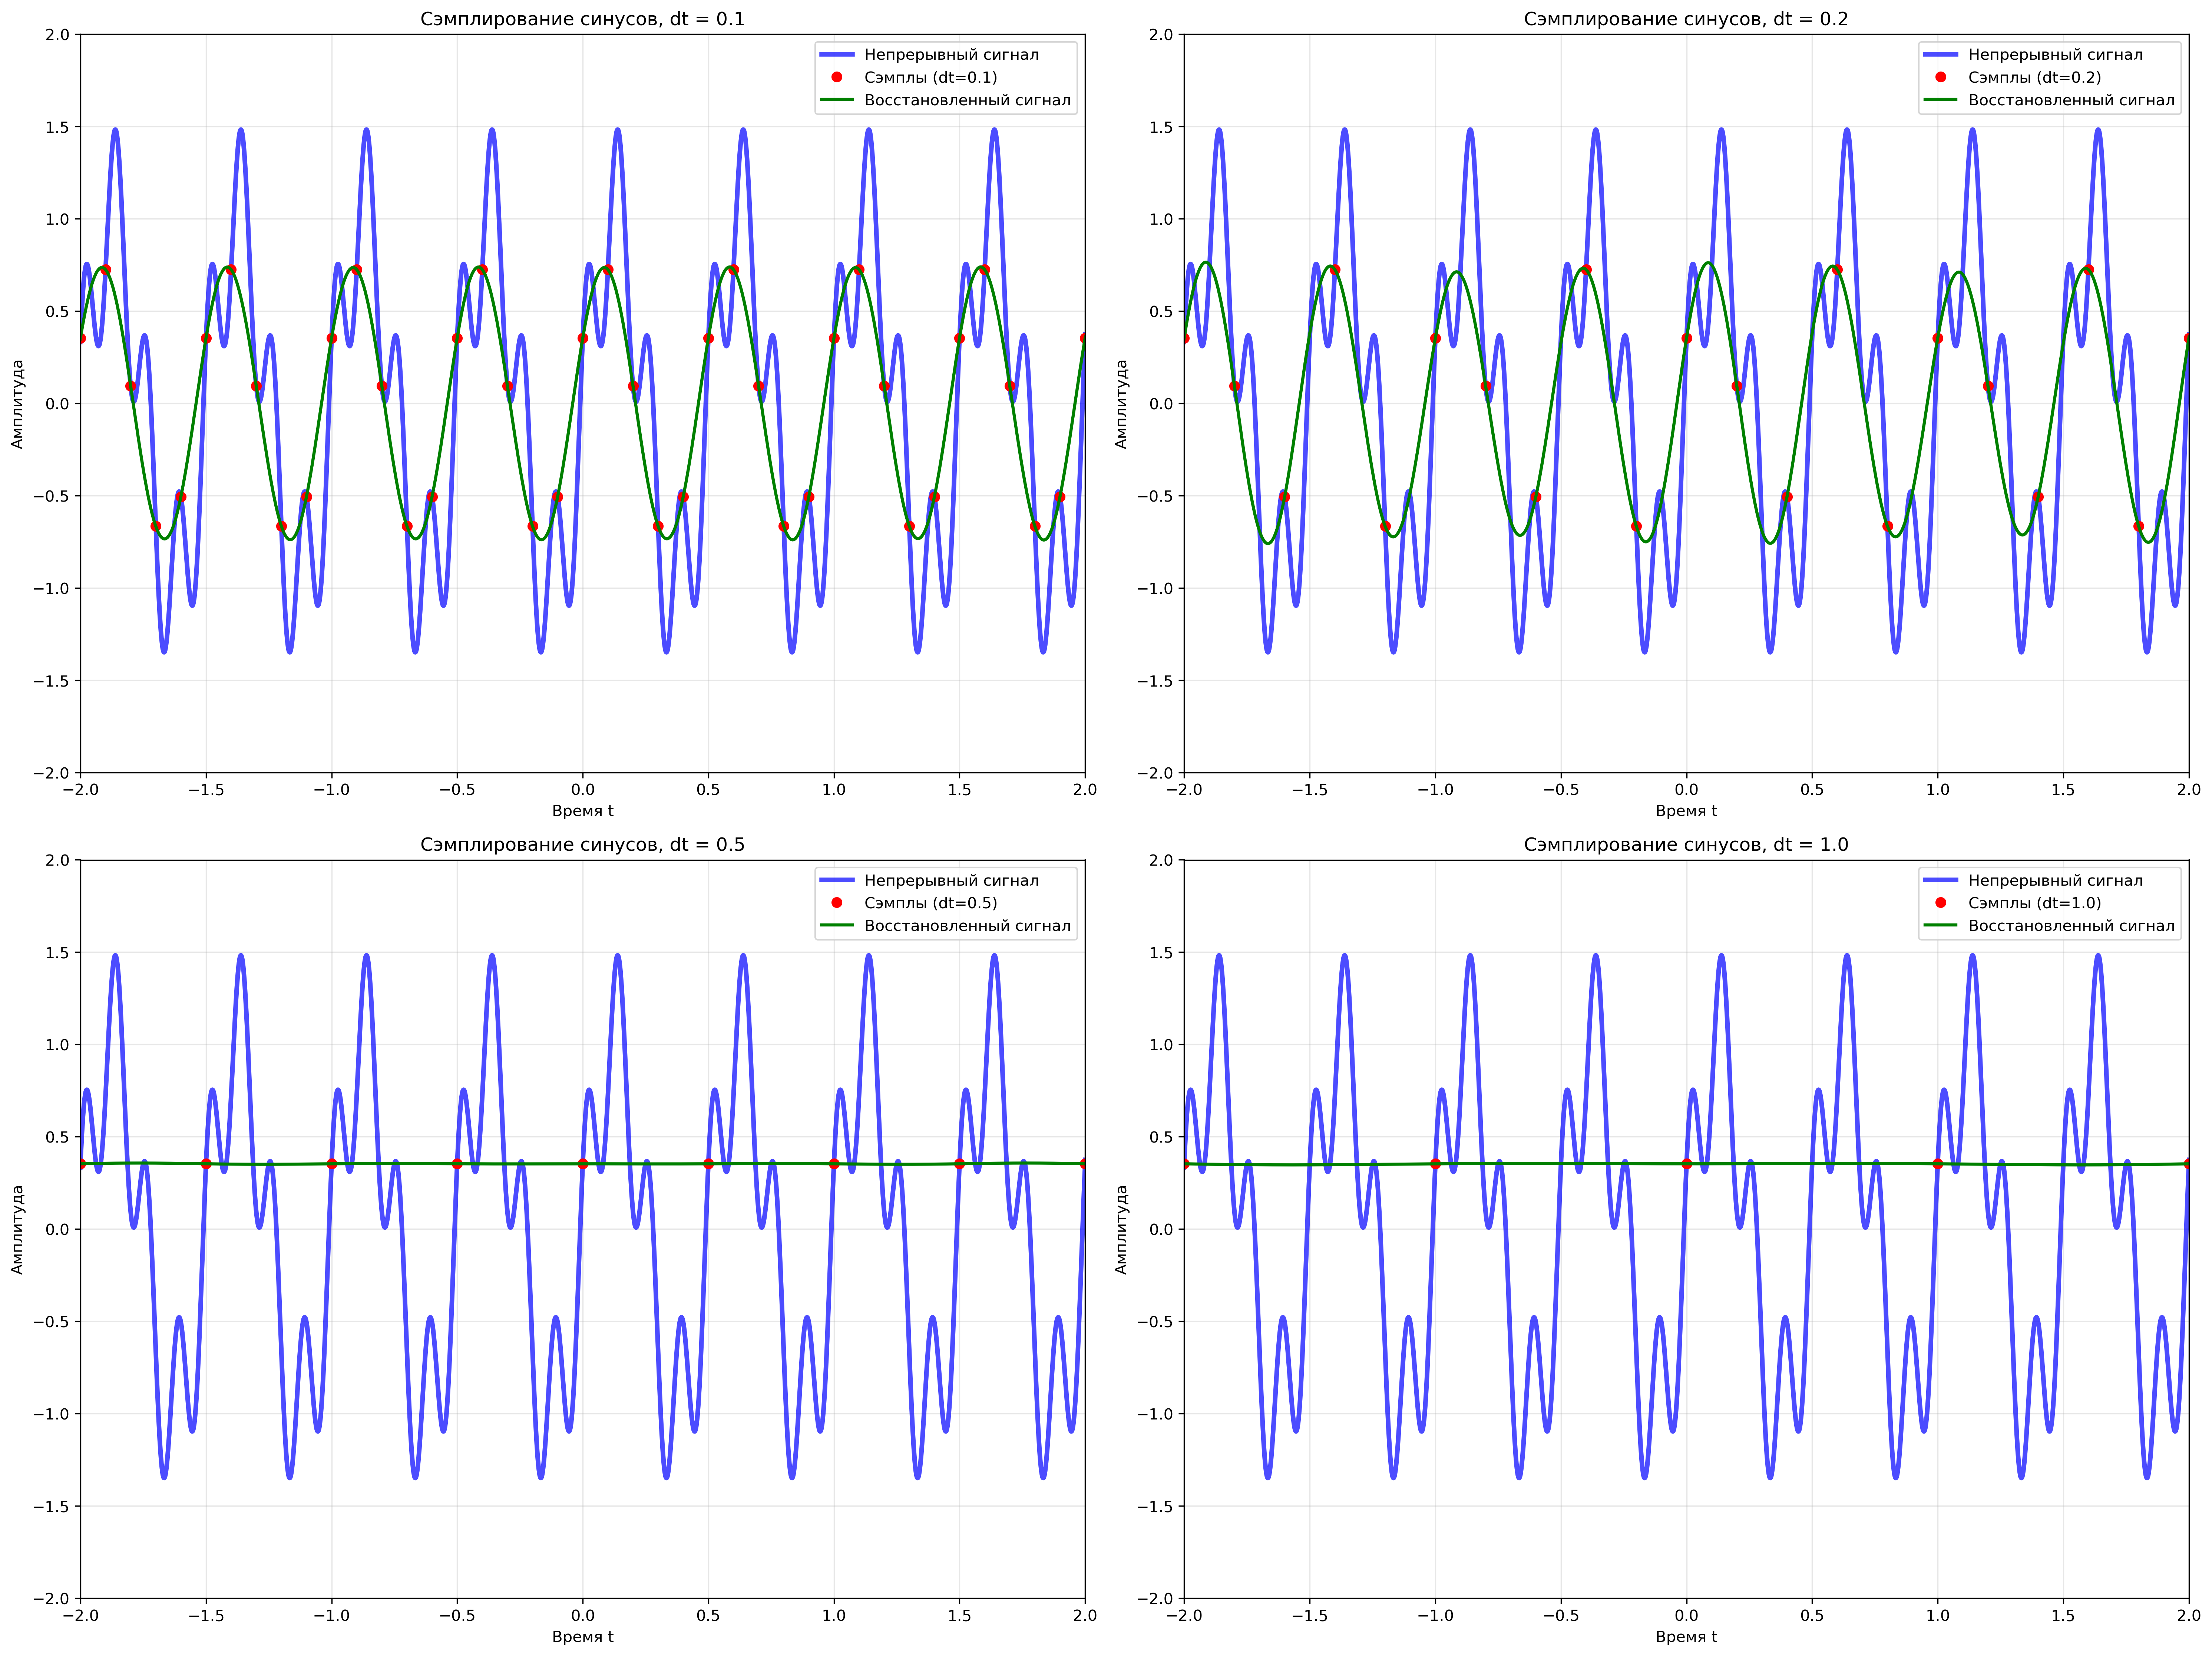
\includegraphics[width=0.8\textwidth]{images/task2/sampling_sines.png}
    \caption{Сэмплирование и восстановление суммы синусов при различных шагах дискретизации}
    \label{fig:sampling_sines}
\end{figure}

\begin{figure}[H]
    \centering
    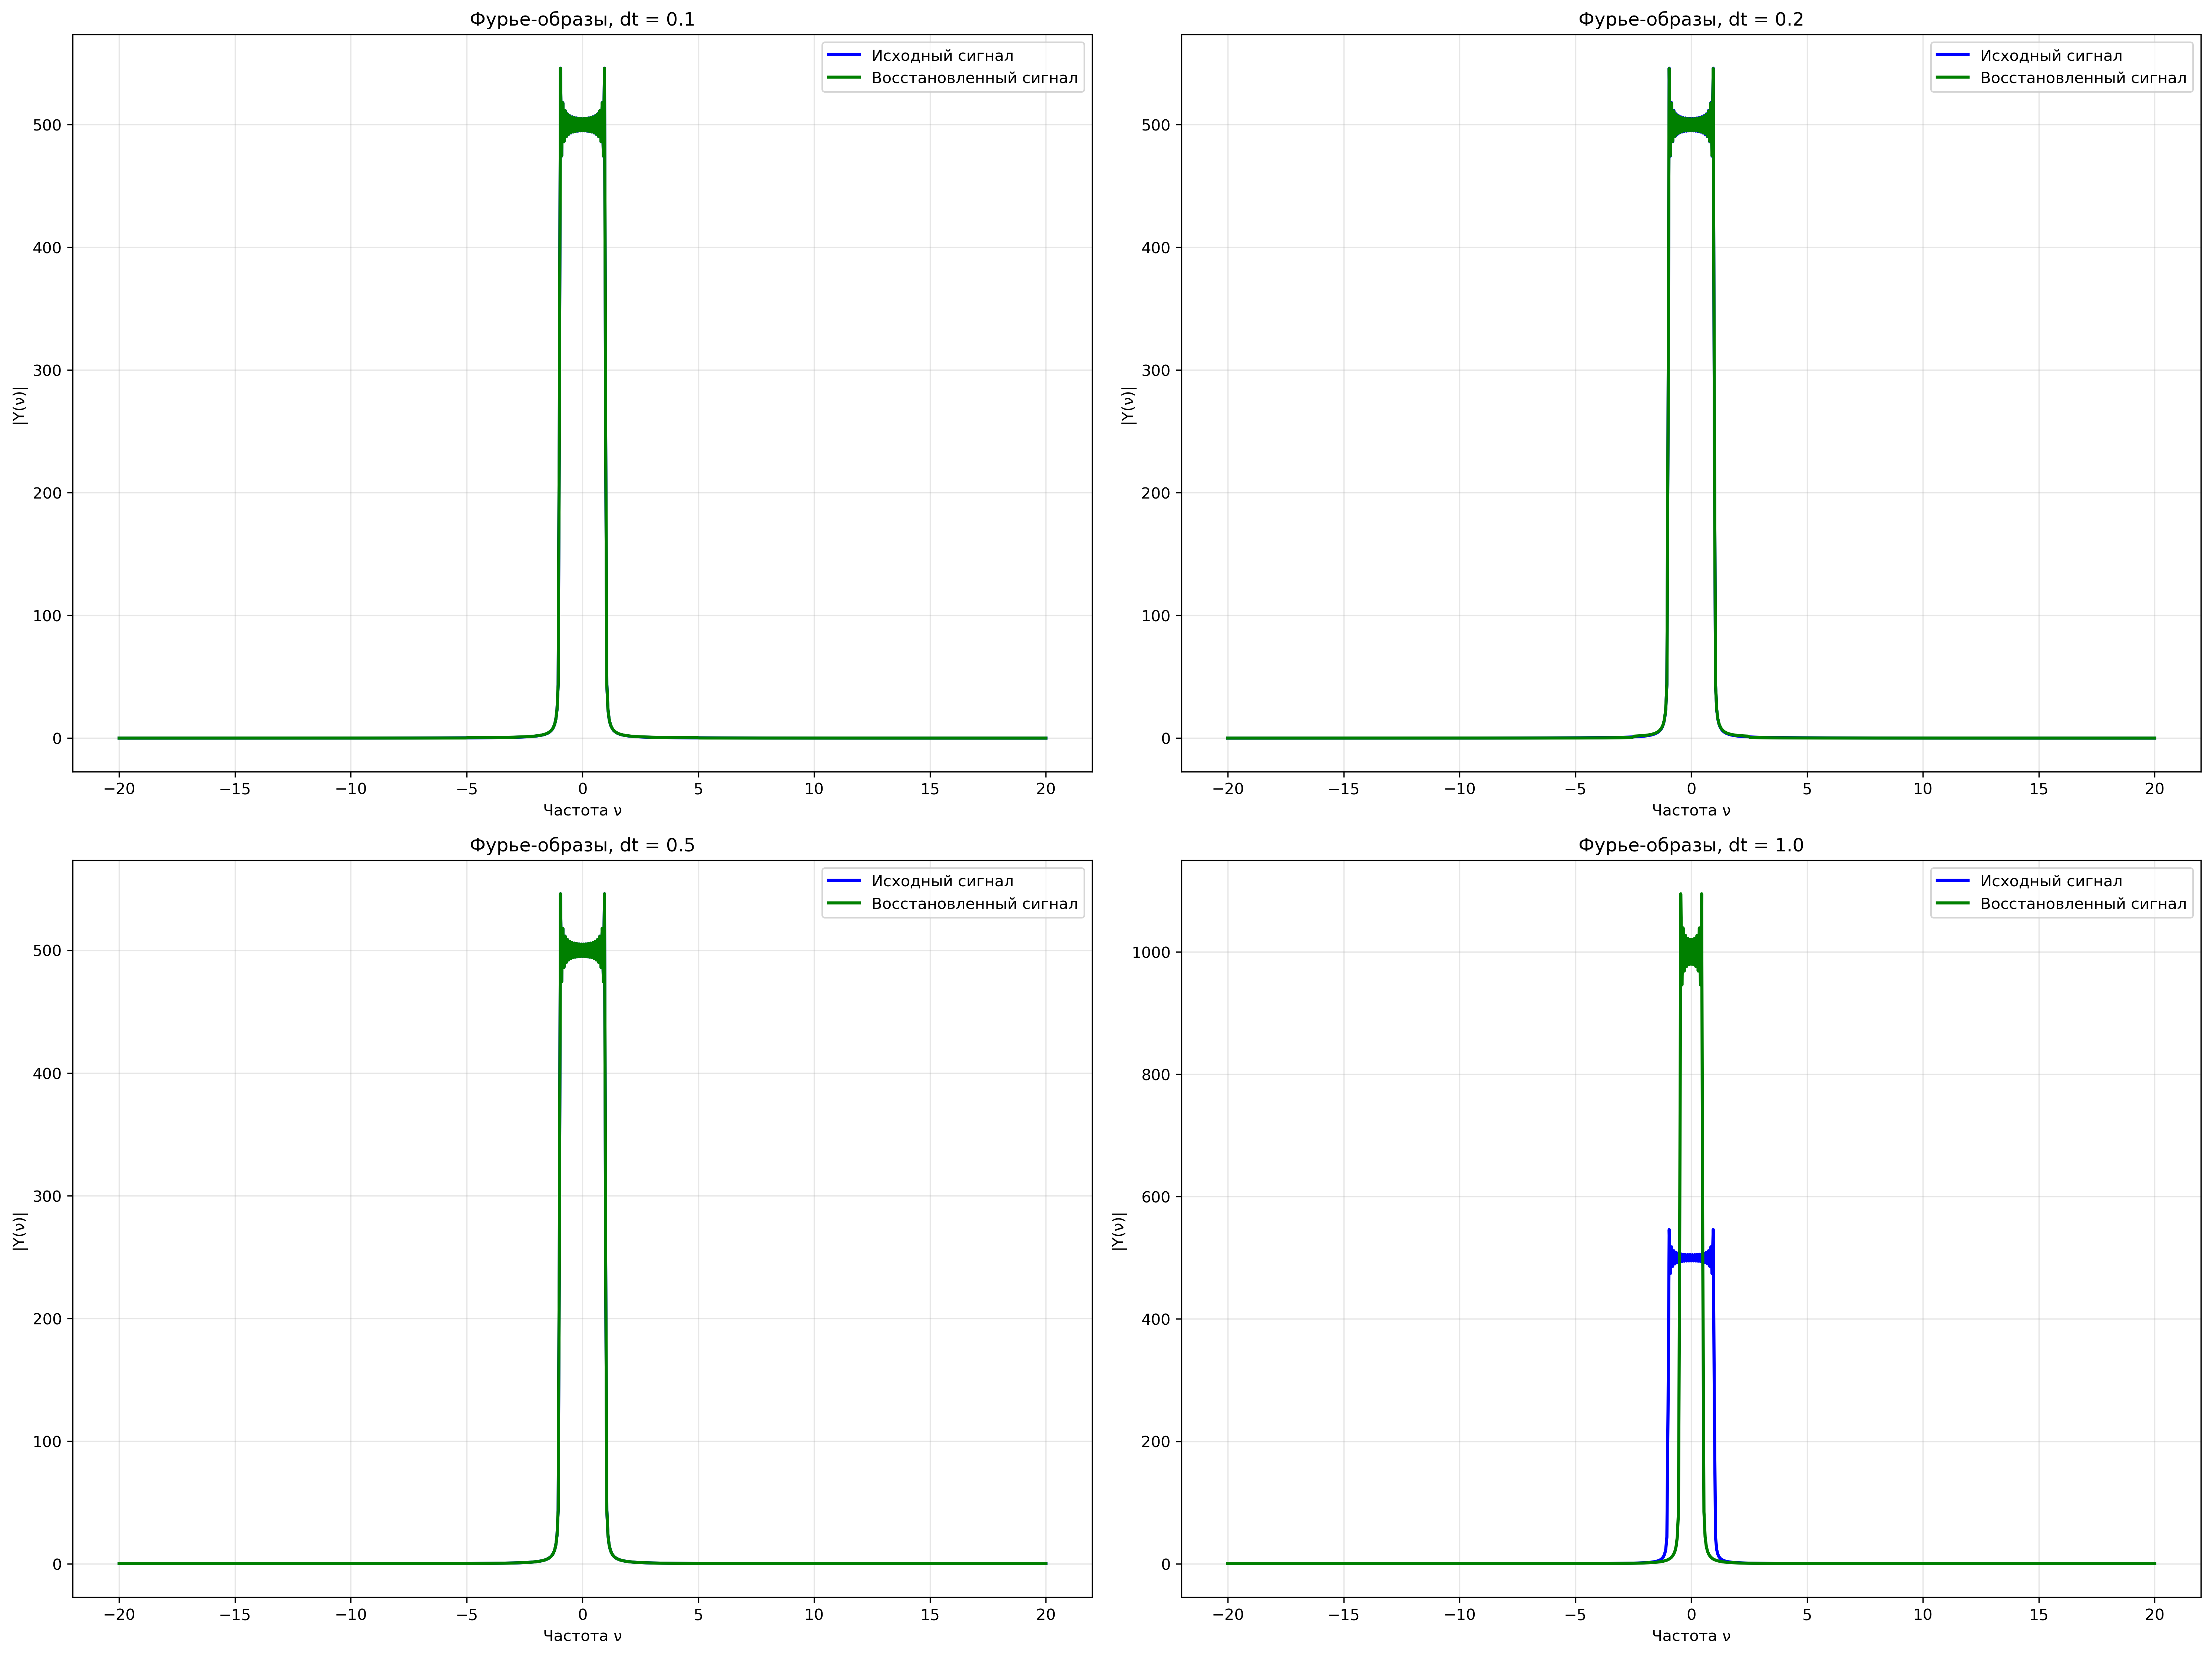
\includegraphics[width=0.8\textwidth]{images/task2/sampling_sinc_fourier.png}
    \caption{Сэмплирование функции sinc и анализ Фурье-образов исходного и восстановленного сигналов}
    \label{fig:sampling_sinc_fourier}
\end{figure}

\begin{figure}[H]
    \centering
    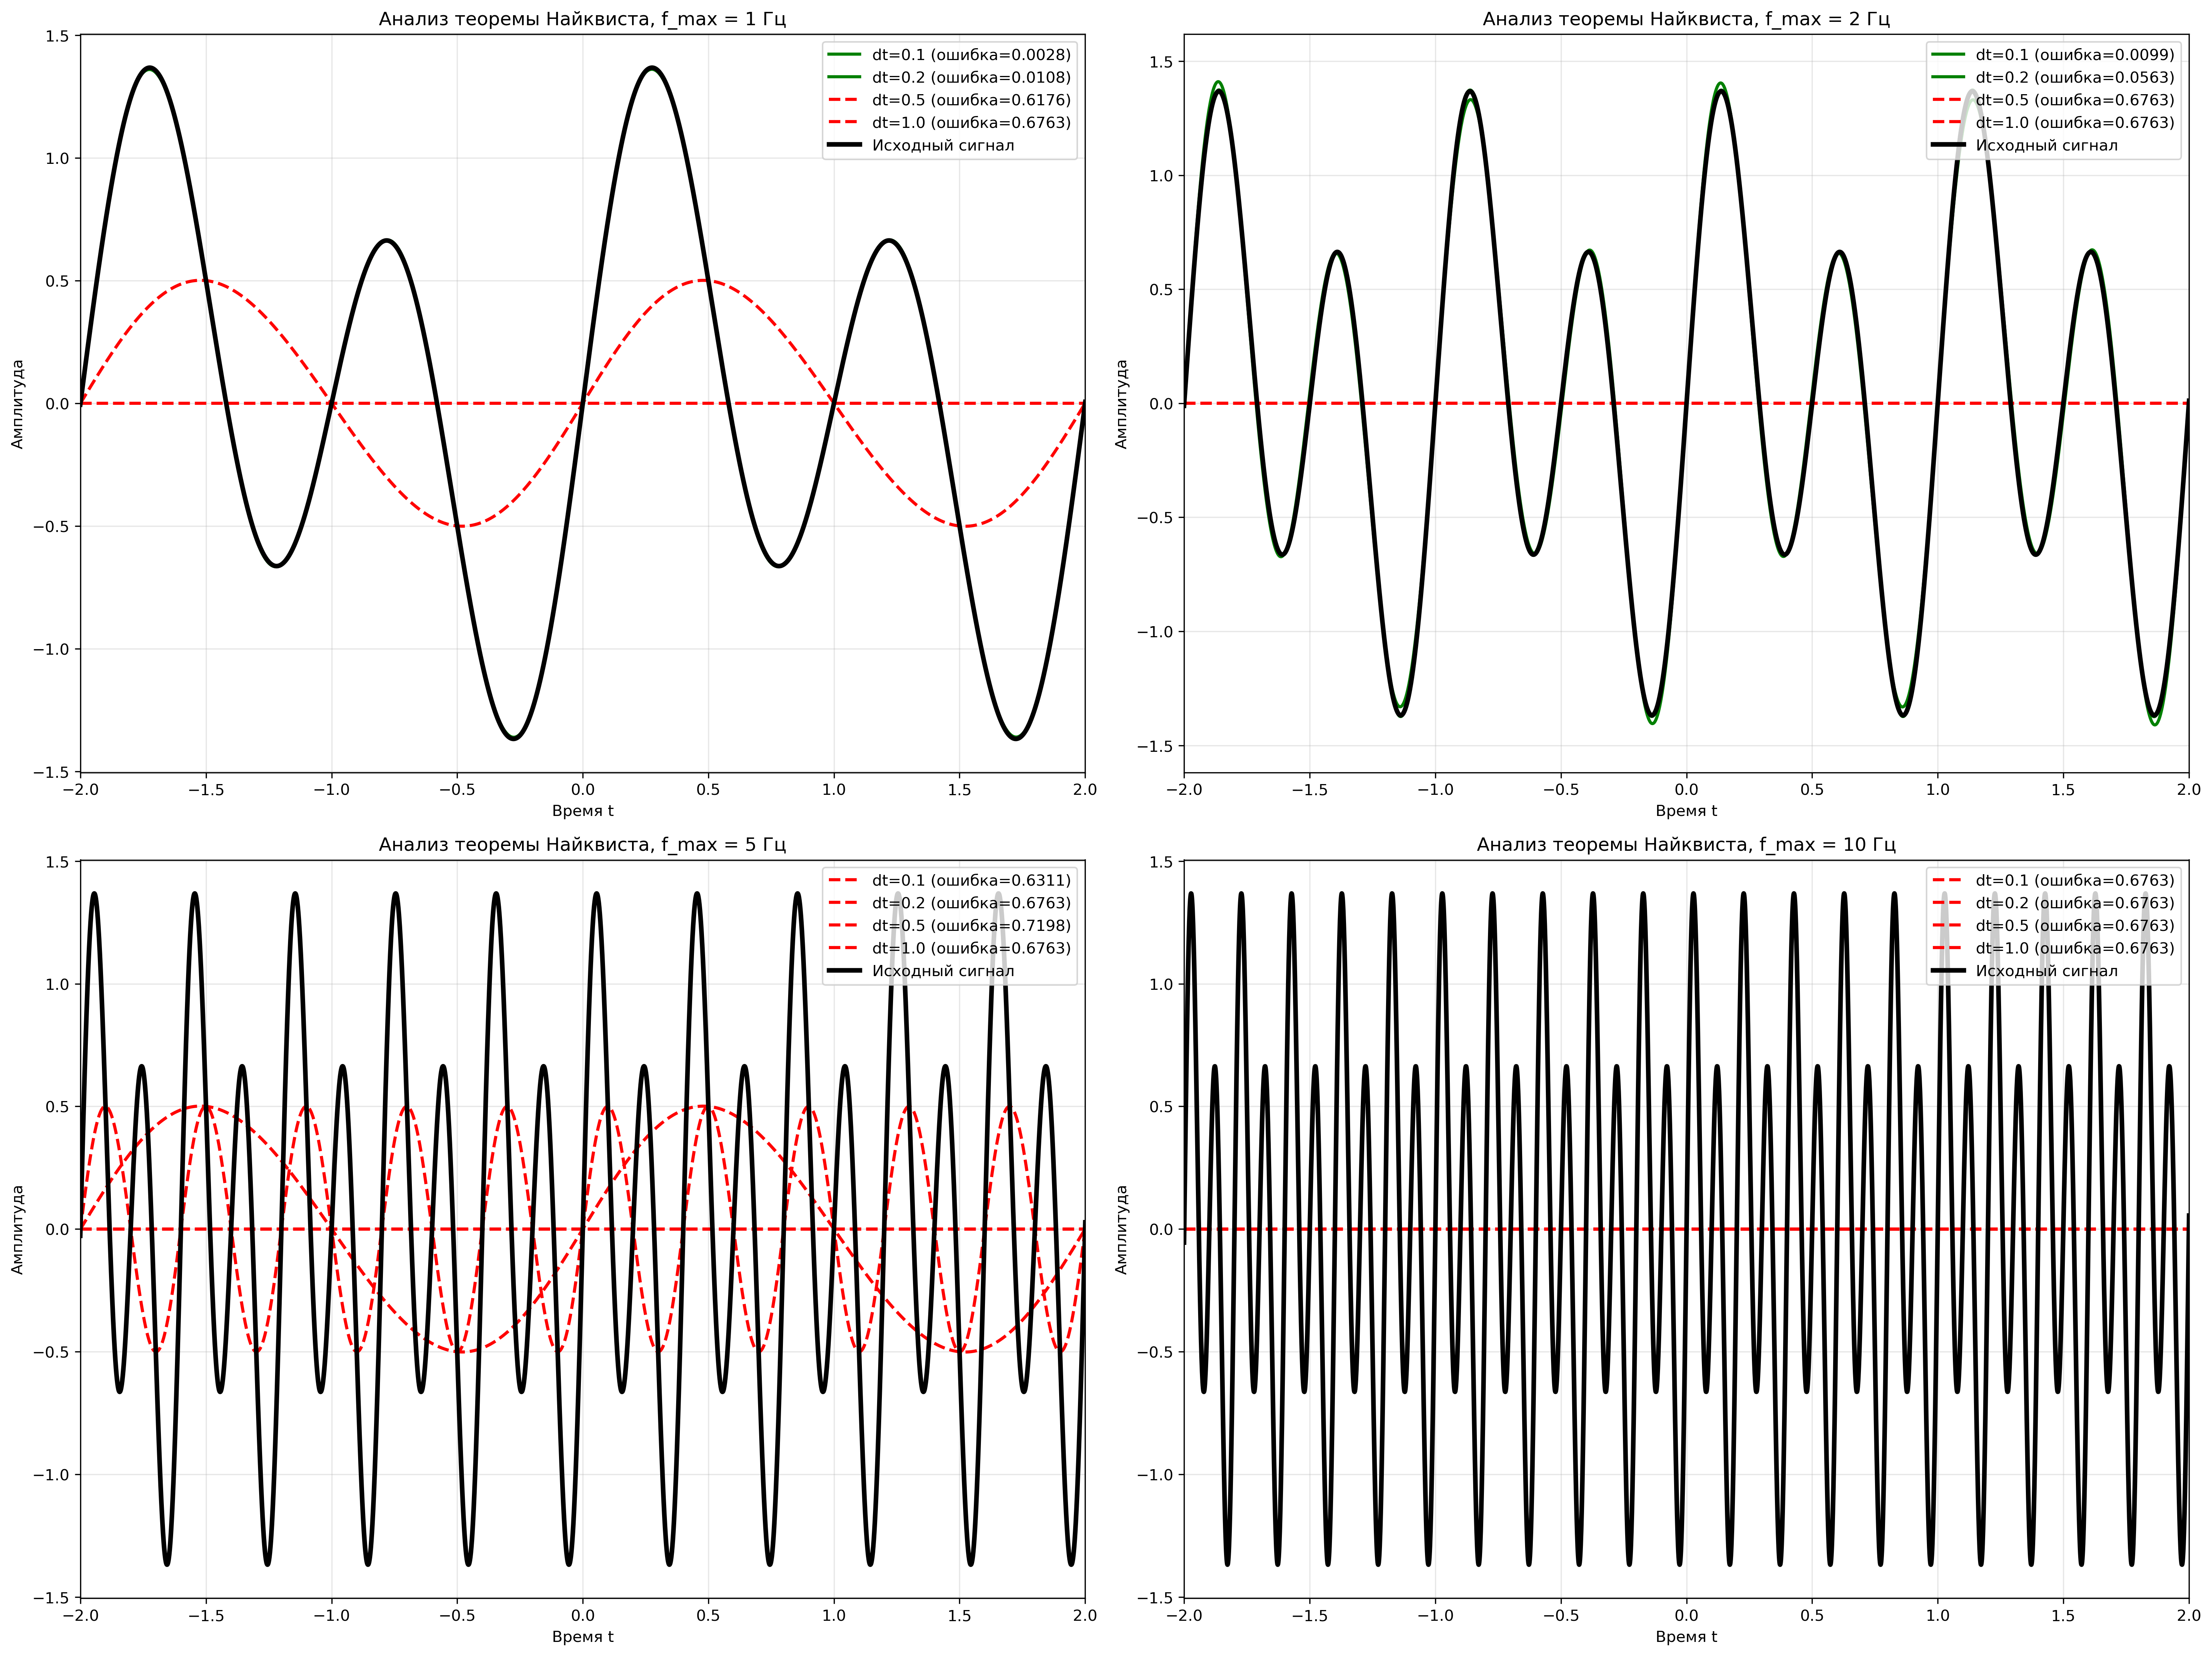
\includegraphics[width=0.8\textwidth]{images/task2/nyquist_analysis.png}
    \caption{Детальный анализ теоремы Найквиста-Шеннона-Котельникова}
    \label{fig:nyquist_analysis}
\end{figure}

\subsection*{Анализ результатов}

\textbf{Сэмплирование синусов:}
\begin{itemize}
    \item \textbf{Параметры:} $a_1 = 1.0$, $a_2 = 0.5$, $f_1 = 2$ Гц, $f_2 = 8$ Гц
    \item \textbf{Максимальная частота:} $f_{max} = 8$ Гц
    \item \textbf{Частота Найквиста:} $f_{Nyquist} = 2 \times 8 = 16$ Гц
    \item \textbf{Результат:} При $dt > 1/16$ с возникают искажения (алиасинг)
\end{itemize}

\textbf{Сэмплирование sinc функции:}
\begin{itemize}
    \item \textbf{Параметр:} $b = 1$, что соответствует $f_{max} = b = 1$ Гц
    \item \textbf{Частота Найквиста:} $f_{Nyquist} = 2$ Гц
    \item \textbf{Результат:} Точное восстановление при $f_{samp} \geq 2$ Гц
\end{itemize}

\textbf{Выводы о теореме Найквиста-Шеннона-Котельникова:}
\begin{enumerate}
    \item \textbf{Условие теоремы:} $f_{samp} > 2f_{max}$ обеспечивает точное восстановление
    \item \textbf{Интерполяция:} Формула $y(t) = \sum_n y[n] \cdot \text{sinc}\left(\frac{t - n \cdot dt}{dt}\right)$ даёт точное восстановление
    \item \textbf{Алиасинг:} При нарушении условий теоремы высокочастотные компоненты "складываются" в низкочастотный диапазон
    \item \textbf{Спектральный анализ:} Фурье-образы исходного и восстановленного сигналов совпадают при выполнении условий теоремы
\end{enumerate}

\section*{Общие выводы}

\begin{enumerate}
    \item \textbf{Методы вычисления Фурье-образа:}
    \begin{itemize}
        \item Численное интегрирование: точное, но медленное
        \item DFT с правильным масштабированием: быстрое и точное (ускорение в 271 раз)
        \item Ключ к успеху DFT — правильное масштабирование на $dt$
    \end{itemize}
    
    \item \textbf{Важность комплексного анализа:}
    \begin{itemize}
        \item Сравнение только модулей образов недостаточно
        \item Необходимо анализировать действительную и мнимую части отдельно
        \item Это выявляет тонкие различия между методами
    \end{itemize}
    
    \item \textbf{Теорема сэмплирования:}
    \begin{itemize}
        \item Подтверждается экспериментально на различных примерах
        \item Критически важна для цифровой обработки сигналов
        \item Интерполяция sinc функцией обеспечивает теоретически точное восстановление
    \end{itemize}
    
    \item \textbf{Практические рекомендации:}
    \begin{itemize}
        \item Использовать DFT с правильным масштабированием для быстрых вычислений
        \item Всегда проверять соответствие теореме Найквиста при сэмплировании
        \item Анализировать комплексные образы, а не только их модули
    \end{itemize}
\end{enumerate}